\subsection{Teil IV. Fortgeschrittene Konvergenz und Feinabstimmung}
\label{subsec:Advanced_Convergence_and_Fine_Tuning}


Die vierte und letzte Phase des Lernprozesses zeichnete sich durch eine langsame, aber stetige Annäherung des Akteurs an das Optimum aus \ref{fig:advanced_convergence_morpheus}. Die Verhaltensänderungen wurden feiner und gezielter, was darauf hindeutet, dass das Modell begann, die subtilen Nuancen der Umgebung zu verstehen und seine Aktionen entsprechend anzupassen. Es war ein langsamer Prozess der Verfeinerung, der darauf abzielte, die optimalen Einstellungen zu finden. Interessanterweise war in dieser Phase auch eine gelegentliche Divergenz bei einem der Agenten zu beobachten. \ref{fig:phase 2 whole lern process} Dies könnte darauf hinweisen, dass trotz der allgemeinen Tendenz zur Konvergenz immer noch das Potential für Instabilitäten oder für das Erkunden von neuen, unerwarteten Lösungspfaden bestand.


\begin{table}[htbp]
\centering
\caption{Stichprobe des Modells Morpheus bei Iteration 6000}
\label{tab:sample_morpheus_6000}
\begin{tabular}{l c}
\hline
\textbf{Parameter} & \textbf{Wert} \\
\hline
Iteration & 6000 \\
Belohnung & -10.21 \\
Aktion & [634.09879804, 55.28446324, 2.65851244] \\
Induktivität & \( 5.0 \times 10^{-3} \) \\
Kapazität & \( 10.0 \times 10^{-6} \) \\
\hline
\end{tabular}
\end{table}

Mit weiteren Fortschritten im Trainingsprozess erreicht das Modell Morpheus nach 6000 Iterationen eine Phase, in der eine signifikante Konvergenz erkennbar ist. Die Belohnungswerte verbessern sich weiter, und die Ausgangsspannung nähert sich stabil der Referenzspannung an, ohne die Versorgungsspannung zu überschreiten \ref{fig:advanced_convergence_morpheus}. Die Daten in Tabelle \ref{tab:sample_morpheus_6000} zeigen, dass die Anpassungen des Akteurs zu einer angemessenen Regelungsleistung führen und die Oszillationen der Spannungswerte minimiert werden. Die Ergebnisse dieser Phase sind vielversprechend und lassen auf eine erfolgreiche Anpassung des Modells schließen.

\begin{figure}[htbp]
\centering
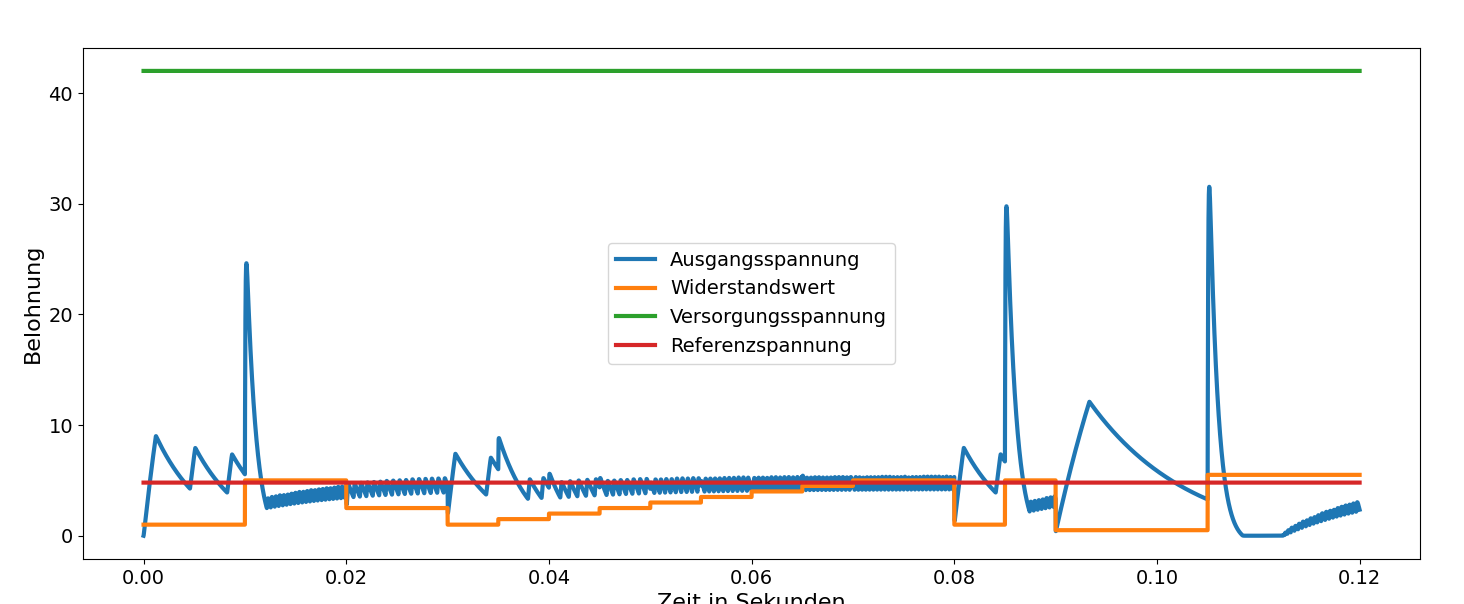
\includegraphics[width=\textwidth, trim=12px 12px 12px 12px, clip]{4Ergebnisse/Phasen/2Phase/TeilIV.png}
\caption{Die fortgeschrittene Konvergenz des Modells Morpheus mit einer sichtbaren Verbesserung der Regelungsleistung. }
\label{fig:advanced_convergence_morpheus}
\end{figure}
